\documentclass[aspectratio=169,usenames,dvipsnames]{beamer}

\usetheme{Madrid}
\usecolortheme{default}
\setbeamertemplate{navigation symbols}{}
\setbeamertemplate{footline}[frame number]

% Packages
\usepackage[utf8x]{inputenc}
\usepackage{amsmath, amsthm, amssymb}
\usepackage{graphicx}
\usepackage{subfigure}
\usepackage{xcolor}
\usepackage{listings}
\usepackage{algorithm}
\usepackage{algorithmic}
\usepackage{hyperref}
\usepackage{diagbox}
\usepackage{multirow}

% Set graphics path
\graphicspath{{../figures/}}

% Define colors
\definecolor{darkblue}{rgb}{0,0,0.5}
\definecolor{darkgreen}{rgb}{0,0.5,0}

% Custom commands
\newcommand{\beq}{\begin{equation*}}
\newcommand{\eeq}{\end{equation*}}
\newcommand{\highlight}[1]{\textcolor{darkblue}{\textbf{#1}}}

% Title Page
\title{Modeling and Implementation of a Photovoltaic Cell Battery Charger System}
\subtitle{Using Fuzzy Logic Control for Maximum Power Point Tracking}
\author{Mehmet Gök}
\institute{Boğaziçi University\\Department of Electrical and Electronics Engineering}
\date{June 4, 2026}

\begin{document}

% ==================== TITLE SLIDE ====================
\frame{\titlepage}

% ==================== OUTLINE ====================
\begin{frame}{Outline}
    \tableofcontents
\end{frame}

% ==================== SECTION 1: INTRODUCTION ====================
\section{Introduction}

\begin{frame}{Motivation: Renewable Energy}
    \begin{itemize}
        \item \highlight{Global energy demand} is rising rapidly due to population growth and industrialization
        \item \highlight{Environmental concerns} with fossil fuels accelerate transition to renewable sources
        \item \highlight{Solar energy} is clean, abundant, and sustainable
        \item \highlight{Photovoltaic (PV) systems} convert sunlight directly into electricity
    \end{itemize}
    
    \vspace{0.3cm}
    \textbf{Challenge:} PV panels have \textcolor{red}{non-linear} power characteristics that vary with:
    \begin{itemize}
        \item \textcolor{red}{Solar irradiance}
        \item \textcolor{red}{Load impedance}
        \item Ambient temperature
    \end{itemize}
\end{frame}

\begin{frame}{Photovoltaic I-V and Power Curves}
    \begin{columns}
        \column{0.5\textwidth}
        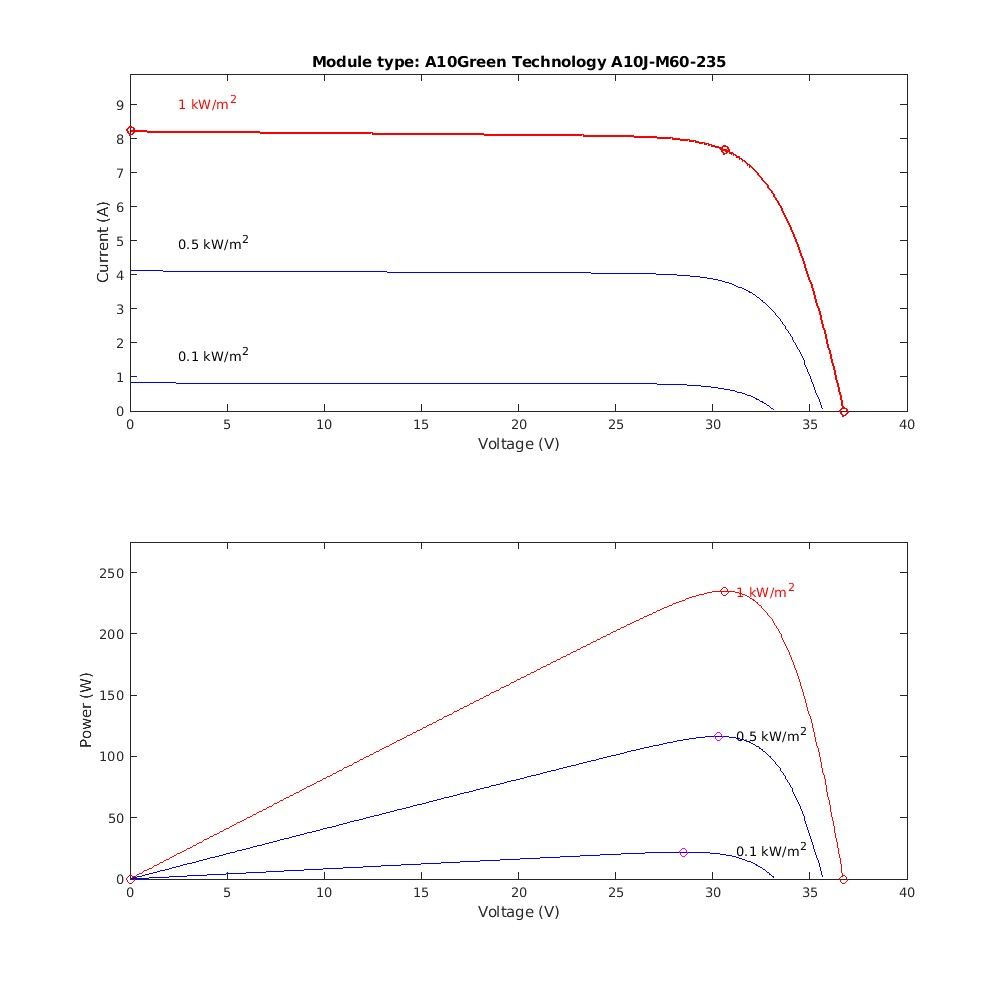
\includegraphics[width=0.95\textwidth]{introduction/pv_IV&powercurves.jpg}
        
        \column{0.5\textwidth}
        \highlight{Key Insight:} There exists a unique operating point (MPP) where the PV panel produces \textcolor{red}{maximum power}
        
        \vspace{0.3cm}
        As irradiance and temperature change, the MPP \textcolor{red}{shifts}
        
        \vspace{0.3cm}
        \textbf{Solution:} Dynamically adjust the load impedance to keep the panel at MPP
    \end{columns}
\end{frame}

\begin{frame}{MPPT Algorithms: Comparison}
    \begin{table}
        \centering
        \footnotesize
        \begin{tabular}{|l|c|c|c|c|}
            \hline
            \textbf{Algorithm} & \textbf{Complexity} & \textbf{Accuracy} & \textbf{Speed} & \textbf{Cost} \\
            \hline
            P\&O (Perturb \& Observe) & Low & Medium & Medium & Low \\
            \hline
            IncCond (Incremental Cond.) & Medium & High & High & Medium \\
            \hline
            Standard FLC & High & High & High & High \\
            \hline
            \highlight{Proposed Optimized FLC} & \highlight{Medium} & \highlight{High} & \highlight{High} & \highlight{Low} \\
            \hline
        \end{tabular}
    \end{table}
    
    \vspace{0.3cm}
    \textbf{Our Choice:} \highlight{Fuzzy Logic Controller (FLC)} because:
    \begin{itemize}
        \item \textbf{Robust} against parameter variations and noise
        \item \textbf{Fast convergence} under changing conditions
        \item \textbf{No complex math model} required
        \item \textbf{Reduced oscillations} around MPP (important for battery charging)
    \end{itemize}
\end{frame}

\begin{frame}{Proposed System Architecture}
    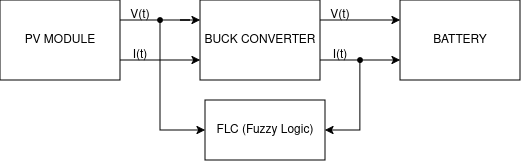
\includegraphics[width=0.8\textwidth]{introduction/system_overview.drawio.png}
    
    \vspace{0.2cm}
    \textbf{Key Innovation:} Replace hardware-intensive arithmetic operations with:
    \begin{itemize}
        \item \textcolor{darkgreen}{Look-Up Tables (LUTs)} instead of multipliers/dividers
        \item \textcolor{darkgreen}{Bitwise shifts} for efficient computation
    \end{itemize}
    
    \vspace{0.2cm}
    \textbf{Result:} Significantly reduced silicon footprint suitable for ASIC implementation
\end{frame}

% ==================== SECTION 2: MATLAB MODEL ====================
\section{Matlab Model}

\begin{frame}{Matlab/Simulink Environment}
    
\includegraphics[width=0.8\textwidth]{matlab/matlab_model_overview.png}
    
    \vspace{0.2cm}
    \textbf{Advantages:}
    \begin{itemize}
        \item High-fidelity Simscape power electronics models
        \item Built-in Photovoltaic Array block with environmental parameter support
        \item Fuzzy Logic Toolbox for intuitive FIS design
        \item Rapid prototyping and parameter tuning
    \end{itemize}
\end{frame}

\begin{frame}{PV Cell Model}
    \textbf{Five-Parameter Model (De Soto et al.):}
    \begin{columns}
        \column{0.55\textwidth}
        \begin{itemize}
            \item Light-generated current: $I_L$
            \item Diode saturation current: $I_0$
            \item Ideality factor: $n$
            \item Series resistance: $R_s$
            \item Shunt resistance: $R_{sh}$
        \end{itemize}
        
        \column{0.45\textwidth}
        \centering
        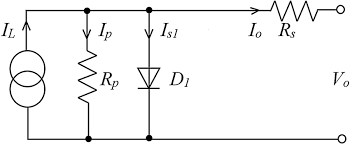
\includegraphics[width=0.95\textwidth]{five_parameter.png}
    \end{columns}
    
    \vspace{0.4cm}
    \textbf{Dynamic I-V Relationship:}
    \begin{itemize}
        \item Accurately reproduces non-linear panel behavior across varying irradiance and temperature conditions.
    \end{itemize}
\end{frame}

\begin{frame}{PV Panel Specifications}
    \textbf{Modeled Panel Parameters:}
    
    \vspace{0.3cm}
    \begin{table}
        \centering
        \begin{tabular}{|l|c|}
            \hline
            \textbf{Parameter} & \textbf{Value} \\
            \hline
            Maximum Power ($P_{mpp}$) & 235 W \\
            \hline
            Open Circuit Voltage ($V_{oc}$) & 36.72 V \\
            \hline
            Short Circuit Current ($I_{sc}$) & 8.23 A \\
            \hline
            MPP Voltage ($V_{mpp}$) & 30.6 V \\
            \hline
        \end{tabular}
    \end{table}
\end{frame}

\begin{frame}{Buck Converter Design}
    \textbf{Challenge:} Step down from $V_{mpp} \approx 30V$ (PV) to $V_{battery} = 12V$
    
    \vspace{0.3cm}
    \begin{table}
        \centering
        \footnotesize
        \begin{tabular}{|l|c|}
            \hline
            \textbf{Parameter} & \textbf{Value} \\
            \hline
            Input Voltage (MPP) & 30.6 V \\
            \hline
            Output Voltage (Battery) & 14.4 V \\
            \hline
            Switching Frequency & 500 kHz \\
            \hline
            Inductance ($L$) & 2.6 $\mu$H \\
            \hline
            Input Capacitance ($C_{in}$) & 47 $\mu$F \\
            \hline
            Converter Efficiency & $\approx$ 95\% \\
            \hline
        \end{tabular}
    \end{table}
    
    \vspace{0.2cm}
    The duty cycle is adjusted by the FLC to vary effective load impedance and track MPP
\end{frame}

\begin{frame}{Fuzzy Logic Controller: Overview}
    
\includegraphics[width=0.65\textwidth]{matlab/fuzzy_controller_block_diagram.png}
    
    \vspace{0.2cm}
    \textbf{Sugeno-type FIS:} Computationally efficient for digital implementation
\end{frame}

\begin{frame}{FLC: Sampling and Inputs}
    \textbf{Sampling Frequency:} $f_s = 20$ kHz (40x slower than switching frequency)
    
    \vspace{0.2cm}
    \textbf{ADC Resolution:} 10-bit $\rightarrow 2^{10} = 1024$ levels
    
    \vspace{0.3cm}
    \textbf{Three Control Inputs:}
    \begin{enumerate}
        \item \highlight{$dV$} - Change in PV voltage between samples
        \item \highlight{$dI$} - Change in PV current between samples
        \item \highlight{$V_{pv}$} - Instantaneous PV voltage (determines operating region)
    \end{enumerate}
    
    \vspace{0.3cm}
    \textbf{Process Pipeline:}
    \begin{itemize}
        \item \textcolor{darkgreen}{Fuzzification} $\rightarrow$ Convert crisp values to linguistic variables
        \item \textcolor{darkgreen}{Rule Evaluation} $\rightarrow$ Apply linguistic rules
        \item \textcolor{darkgreen}{Defuzzification} $\rightarrow$ Generate crisp control output
    \end{itemize}
\end{frame}

\begin{frame}{FLC: Membership Functions}
    \textbf{Input Variables:}
    \begin{itemize}
        \item $dV$, $dI$: \texttt{Negative, Zero, Positive}
        \item $V_{pv}$: \texttt{Low\_Voltage, Optimal\_Range, High\_Voltage}
    \end{itemize}
    
    \vspace{0.2cm}
    \textbf{Output Variable ($\Delta D$):}
    \[\text{\texttt{Big\_Decrease}(-15), \texttt{Decrease}(-1), \texttt{Hold}(0), \texttt{Increase}(+1), \texttt{Big\_Increase}(+15)}\]
    
    \vspace{0.3cm}
    \textbf{MPP Calculations (10-bit ADC, 40V reference):}
    \[\text{ADC\_count} = \frac{V}{40V} \times 1024\]
    
    \begin{itemize}
        \item MPP: 30.6V $\rightarrow$ ADC count $\approx 783$
        \item Low Voltage threshold: 28.5V $\rightarrow$ count $\approx 730$
        \item High Voltage threshold: 32.8V $\rightarrow$ count $\approx 840$
    \end{itemize}
\end{frame}

\begin{frame}{FLC: Rule Base}
    \textbf{Two-Tier Control Strategy:}
    
    \vspace{0.2cm}
    \begin{columns}
        \column{0.45\textwidth}
        \textbf{1. Safety Rules (far from MPP):}
        
        \vspace{0.1cm}
        {\footnotesize
        \begin{tabular}{|c|c|}
            \hline
            \textbf{PV Voltage ($V_{pv}$)} & \textbf{Output ($\Delta D$)} \\
            \hline
            \texttt{Low\_Voltage} & \texttt{Big\_Decrease} \\
            \hline
            \texttt{High\_Voltage} & \texttt{Big\_Increase} \\
            \hline
        \end{tabular}
        }
        
        \vspace{0.3cm}
        \textbf{2. Fine-Tuning Rules (near MPP):}
        
        \vspace{0.1cm}
        {\footnotesize
        \begin{tabular}{|c|c|c|c|}
            \hline
            \diagbox{$dI$}{$dV$} & \textbf{Negative} & \textbf{Zero} & \textbf{Positive} \\
            \hline
            \textbf{Negative} & \texttt{Decrease} & \texttt{Hold} & \texttt{Increase} \\
            \hline
            \textbf{Zero} & \texttt{Hold} & \texttt{Hold} & \texttt{Hold} \\
            \hline
            \textbf{Positive} & \texttt{Increase} & \texttt{Hold} & \texttt{Decrease} \\
            \hline
        \end{tabular}
        }
        
        \column{0.65\textwidth}
        \centering
        
\includegraphics[width=0.95\textwidth]{pv_IV&powercurves.jpg}
    \end{columns}
\end{frame}

\begin{frame}{FLC: Duty Cycle Integration}
    \textbf{Bumpless Transfer Mechanism:}
    \[D[n] = D[n-1] + \frac{\Delta D}{16384}\]
    
    \vspace{0.3cm}
    \textbf{Benefits:}
    \begin{itemize}
        \item Prevents discontinuities when switching between control states
        \item Provides damping effect and reduces oscillations
        \item Makes system robust against noise
        \item Fine control granularity
    \end{itemize}
    
    \vspace{0.3cm}
    \textbf{Critical Rule:} If both $dV = 0$ and $dI = 0$, hold duty cycle constant
    $\rightarrow$ Prevents oscillations at power peak
\end{frame}

\begin{frame}{MATLAB Simulation: Results Overview}
    \vspace*{-0.2cm}
    \begin{columns}[c]
        
        \begin{column}{0.78\textwidth}
            \centering
            % trim={<left> <bottom> <right> <top>} in centimeters or inches
            % Adjust these numbers slightly if it cuts into your y-axis labels!
            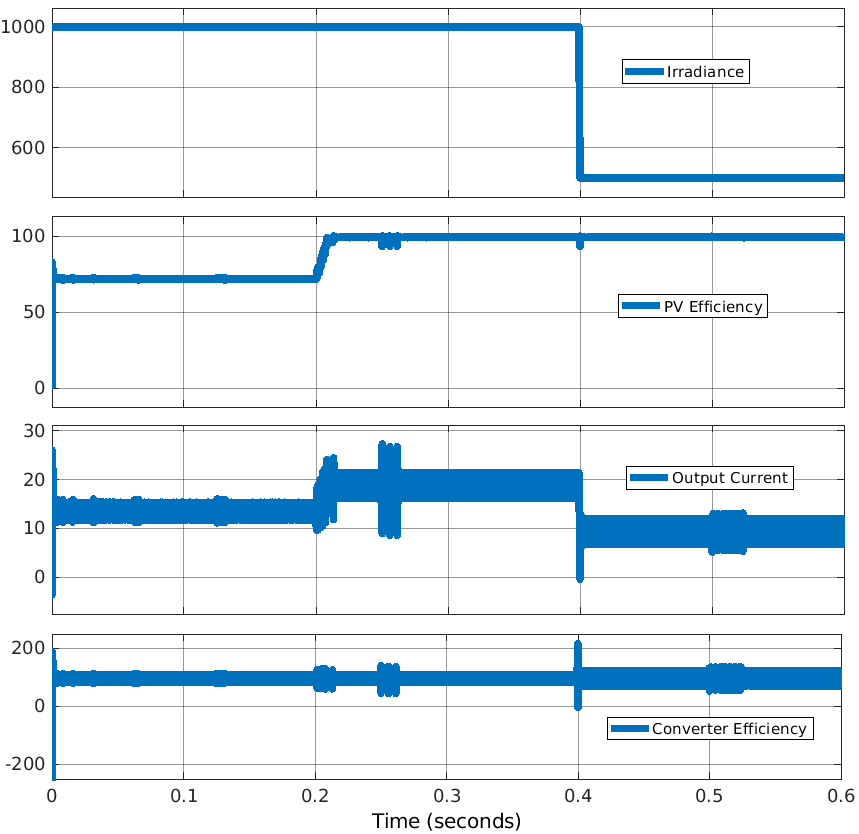
\includegraphics[trim=2cm 0cm 2cm 0cm, clip, width=\textwidth, height=0.76\textheight, keepaspectratio]{matlab/matlabsimresult.jpg}
        \end{column}
        
        \begin{column}{0.20\textwidth}
            \raggedright
            \small
            \textbf{Simulation Stats:}
            \vspace{0.15cm}
            \begin{itemize}
                \item \textbf{Duration:} 0.6s
                \item \textbf{Efficiency:} $\approx 95\%$
            \end{itemize}
        \end{column}
        
    \end{columns}
\end{frame}

\begin{frame}{MATLAB Simulation: Three Phases}
    \textbf{Phase 1 - Initial Stabilization (0-0.2s):}\vspace{-0.05cm}
    \begin{itemize}
        \item Fixed duty cycle, FLC inactive
    \end{itemize}
    
    \vspace{0.08cm}
    \textbf{Phase 2 - FLC Activation (0.2s):}\vspace{-0.05cm}
    \begin{itemize}
        \item \highlight{99\% efficiency in 13.4 ms}
    \end{itemize}
    
    \vspace{0.08cm}
    \textbf{Phase 3 - Transient Response (0.4s):}\vspace{-0.05cm}
    \begin{itemize}
        \item Rapid recovery: \highlight{99\% in $\approx 1$ ms}
    \end{itemize}
\end{frame}

\begin{frame}{MATLAB Simulation: Transient Details}
    \begin{columns}
        \column{0.5\textwidth}
        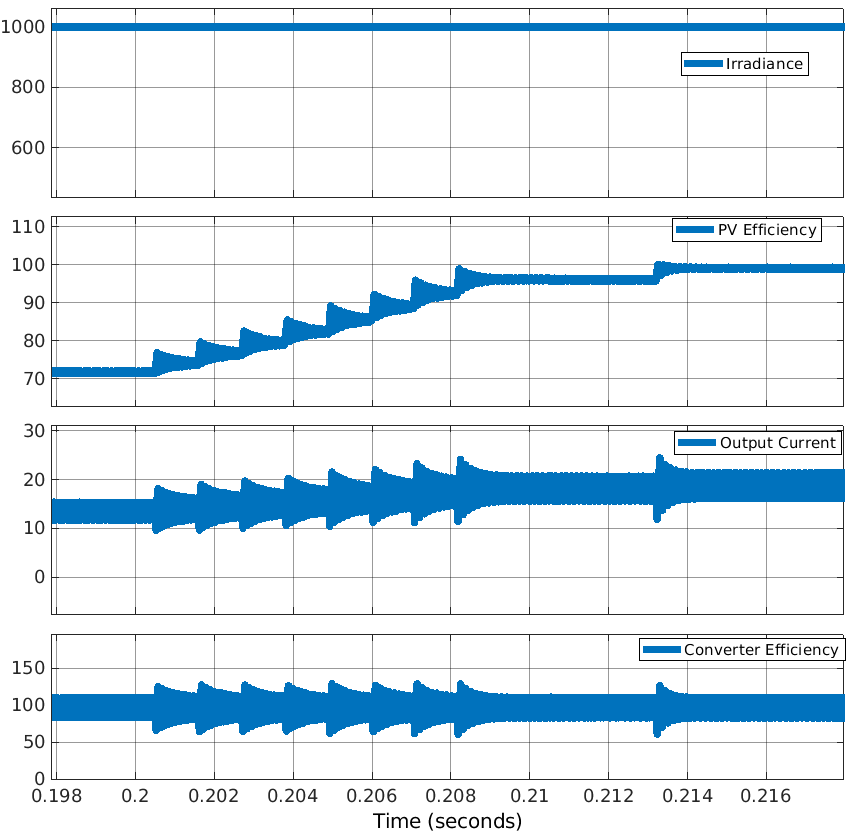
\includegraphics[width=0.85\textwidth]{matlab/matlab_sim_result_around0_2.jpg}
        \small \centering FLC activation
        
        \column{0.5\textwidth}
        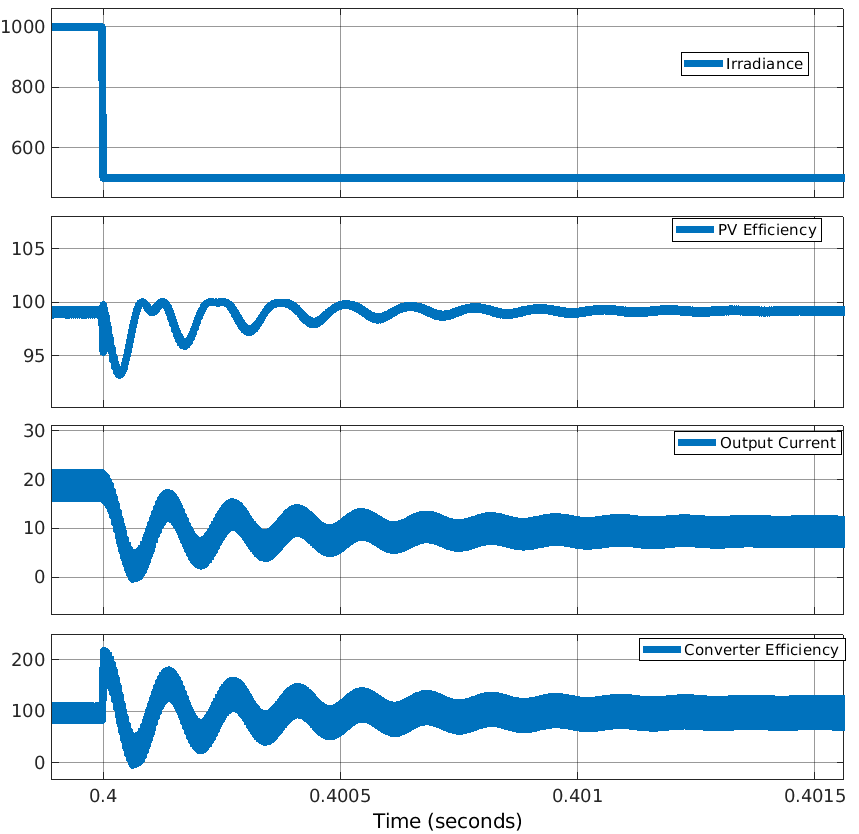
\includegraphics[width=0.85\textwidth]{matlab/matlab_sim_result_around0_4.jpg}
        \small \centering Transient response
    \end{columns}
    
    \vspace{0.15cm}
    \textbf{Key Achievement:} Fast convergence and excellent disturbance rejection
\end{frame}

% ==================== SECTION 3: BEHAVIORAL MODELING ====================
\section{Behavioral Modeling \& System Integration}

\begin{frame}{Migration to Hardware Description}
    \textbf{Challenge:} Bridge MATLAB (high-level) to Silicon (circuit-level)
    
    \vspace{0.3cm}
    \textbf{Solution:} 
    \begin{itemize}
        \item Implement fuzzy controller in \highlight{SystemVerilog}
        \item Model PV panel in \highlight{Verilog-A}
        \item Verify in \highlight{Cadence Virtuoso}
    \end{itemize}
    
    \vspace{0.3cm}
    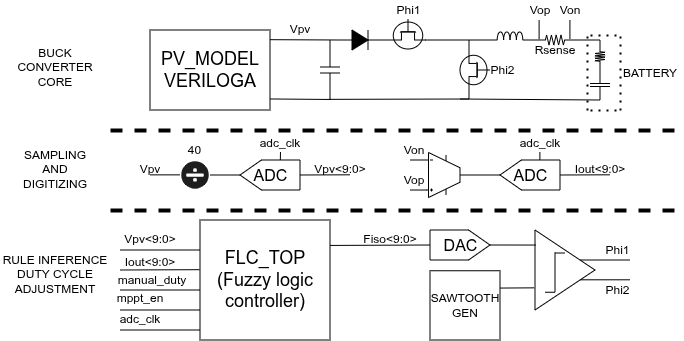
\includegraphics[width=0.55\textwidth]{cadence_model/cadence_system_model.png}
\end{frame}

\begin{frame}{PV Model in Verilog-A}
    \textbf{Behavioral Modeling:}\vspace{-0.1cm}
    \begin{itemize}
        \item Five-parameter model based on De Soto et al.
        \item Takes irradiance and temperature as inputs
        \item Dynamically calculates output current
    \end{itemize}
    
    \vspace{0.1cm}
    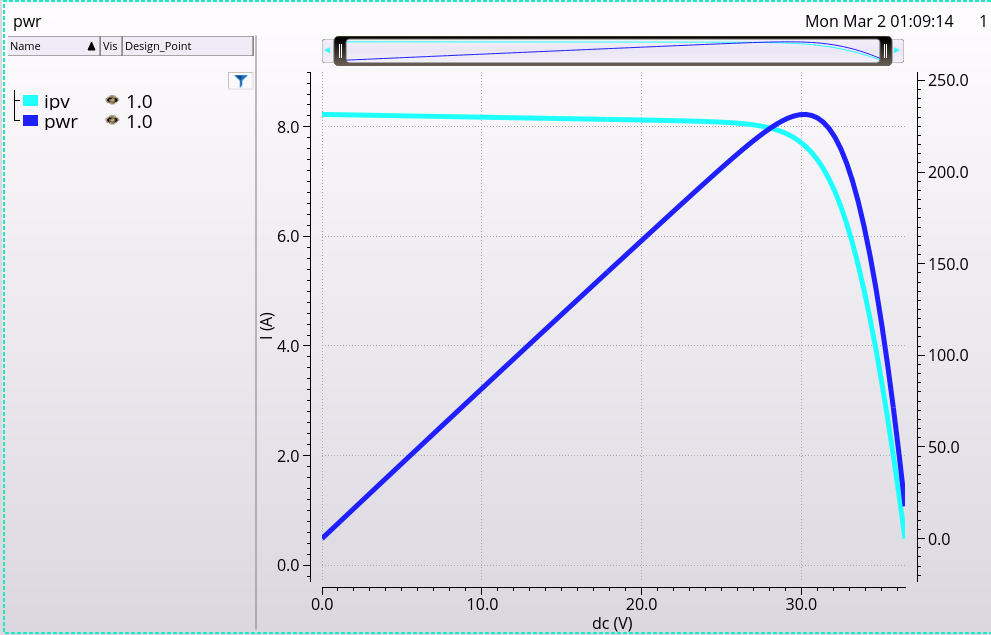
\includegraphics[width=0.48\textwidth]{cadence_model/pvmodel_ivandpower.png}
\end{frame}

% ==================== SECTION 4: ANALOG IMPLEMENTATION ====================
\section{Analog Implementation}

\begin{frame}{Analog Front-End Overview}
    \textbf{Core Analog Blocks:}
    \begin{itemize}
        \item \highlight{Successive Approximation Register (SAR) ADC} - Converts analog signals
        \item \highlight{Bandgap Reference} - Provides stable voltage reference
        \item \highlight{Low Dropout Regulator (LDO)} - Powers digital circuits
        \item \highlight{Capacitive DAC} - Generates reference voltages
    \end{itemize}
    
    \vspace{0.3cm}
    \textbf{Key Design Consideration:}
    \[\text{Minimize silicon area while maintaining measurement accuracy}\]
\end{frame}

\begin{frame}{SAR ADC Architecture}
    \textbf{12-bit SAR ADC Design (10-bit Target ENOB):}
    \begin{itemize}
        \item 12-bit physical resolution with a split CapDAC (6-bit MSB, 6-bit LSB)
        \item Asynchronous, self-timed operation avoids high-frequency clocks
        \item Fully differential topology for high common-mode noise immunity
        \item Provides reliable 10-bit output ($2^{10} = 1024$ levels) for the FLC
    \end{itemize}
    
    \vspace{0.3cm}
    \textbf{Key Performance Metrics:}
    \begin{itemize}
        \item DNL: Differential Non-Linearity
        \item INL: Integral Non-Linearity
        \item ENOB: Effective Number of Bits
        \item SNR: Signal-to-Noise Ratio
    \end{itemize}
\end{frame}

\begin{frame}{Bandgap Reference Circuit}
    \textbf{Purpose:} Generate temperature-stable voltage reference
    
    \vspace{0.2cm}
    \textbf{Design Principles:}
    \begin{itemize}
        \item Temperature coefficient minimization
        \item Process variation robustness
        \item Low power consumption
    \end{itemize}
    
    \vspace{0.3cm}
    \textbf{Typical Output:} $V_{ref} \approx 1.2$ V (technology-dependent)
\end{frame}

\begin{frame}{Power Distribution: LDO Regulator}
    \textbf{Role:} Provide stable low voltage supply for digital circuits
    
    \vspace{0.2cm}
    \textbf{Design Specifications:}
    \begin{itemize}
        \item Low output ripple
        \item Fast transient response to load changes
        \item Efficient area utilization
        \item Wide input voltage range
    \end{itemize}
    
    \vspace{0.3cm}
    \textbf{Typical Configuration:}
    \[\text{Input Voltage} \sim 5\text{V} \rightarrow \text{Output Voltage} \sim 1.8\text{V or } 3.3\text{V}\]
\end{frame}

% ==================== SECTION 5: DIGITAL IMPLEMENTATION ====================
\section{Digital Implementation}

\begin{frame}{Digital Control Architecture}
    \textbf{Core Digital Module:} \highlight{Fuzzy Logic Controller Engine}
    
    \vspace{0.3cm}
    \textbf{Key Optimization:} Replace multipliers/dividers with:
    \begin{itemize}
        \item \textcolor{darkgreen}{Look-Up Tables (LUTs)}
        \item \textcolor{darkgreen}{Bitwise shift operations}
    \end{itemize}
    
    \vspace{0.3cm}
    \textbf{Result:}
    \begin{itemize}
        \item \textbf{Reduced silicon footprint} by $\sim 60-70\%$ vs. arithmetic implementation
        \item \textbf{Lower power consumption}
        \item \textbf{Faster computation}
        \item \textbf{Multiple controllers} can fit on single chip
    \end{itemize}
\end{frame}

\begin{frame}{SystemVerilog Implementation: Fuzzification}
    \textbf{Input Stage:} Convert crisp values to fuzzy membership degrees
    
    \vspace{0.3cm}
    \textbf{Implementation Strategy:}
    \begin{itemize}
        \item \highlight{Piecewise linear} membership functions
        \item \highlight{LUT-based} computation where possible
        \item \highlight{Efficient bit-width} selection (trade-off: area vs. accuracy)
    \end{itemize}
    
    \vspace{0.3cm}
    \textbf{Example:} Triangular membership function
    \[\mu(x) = \begin{cases}
    \frac{x - a}{b - a} & \text{if } a \leq x \leq b \\
    \frac{c - x}{c - b} & \text{if } b \leq x \leq c \\
    0 & \text{otherwise}
    \end{cases}\]
\end{frame}

\begin{frame}{SystemVerilog Implementation: Inference}
    \textbf{Rule Evaluation Stage:} Determine firing strength of each rule
    
    \vspace{0.3cm}
    \textbf{Sugeno System (crisp outputs):}
    \begin{itemize}
        \item Each rule has constant output: $C_i$
        \item Firing strength: $w_i = \mu_1(x_1) \land \mu_2(x_2) \land \mu_3(x_3)$
        \item Use \highlight{bitwise AND} for min operation (very efficient!)
    \end{itemize}
    
    \vspace{0.3cm}
    \textbf{Implementation:}
    \begin{itemize}
        \item Reduced from 27 possible rules down to \highlight{11 total rules}
        \item Hardware implementation further consolidates these into \highlight{8 active weights}
        \item $\mu \land \mu$ implemented via combinational minimum logic (not multipliers)
    \end{itemize}
\end{frame}

\begin{frame}{SystemVerilog Implementation: Defuzzification}
    \textbf{Output Stage:} Generate weighted average control signal
    
    \vspace{0.3cm}
    \textbf{Weighted Average Formula:}
    \[\Delta D = \frac{\sum_{i=1}^{N} w_i \cdot C_i}{\sum_{i=1}^{N} w_i}\]
    
    \vspace{0.3cm}
    \textbf{Hardware-Efficient Approach:}
    \begin{itemize}
        \item Pre-compute numerator: $\sum w_i \cdot C_i$ using LUT or shifts
        \item Denominator: $\sum w_i$ is sum of firing strengths
        \item Division: Use \highlight{right-shift approximation} instead of full divider
    \end{itemize}
    
    \vspace{0.3cm}
    \textbf{Example Shift Trick:} $\frac{x}{16} = x >> 4$ (hardware cost: nearly zero!)
\end{frame}

\begin{frame}{Digital Implementation: Duty Cycle Register}
    \textbf{Integration Block:} Accumulates control decisions
    
    \vspace{0.3cm}
    \[\text{Duty Cycle} = D[n-1] + \frac{\Delta D}{16384}\]
    
    \vspace{0.3cm}
    \textbf{Hardware Implementation:}
    \begin{itemize}
        \item \highlight{Adder} for accumulation
        \item \highlight{Right-shifter} (14 bits) for scaling factor
        \item Saturation logic to keep value in valid range [0, 1]
    \end{itemize}
    
    \vspace{0.3cm}
    \textbf{Output:} PWM signal to buck converter MOSFET driver
\end{frame}

\begin{frame}{Area Optimization Summary}
    \begin{table}
        \centering
        \footnotesize
        \begin{tabular}{|l|c|c|}
            \hline
            \textbf{Operation} & \textbf{Traditional} & \textbf{Optimized} \\
            \hline
            Multiplier (16-bit) & $\sim 5000$ $\mu m^2$ & LUT: $\sim 500$ $\mu m^2$ \\
            \hline
            Divider (16-bit) & $\sim 8000$ $\mu m^2$ & Shift: $\sim 50$ $\mu m^2$ \\
            \hline
            Weighted Average & $\sim 10000$ $\mu m^2$ & $\sim 1500$ $\mu m^2$ \\
            \hline
        \end{tabular}
    \end{table}
    
    \vspace{0.3cm}
    \textbf{Total Estimated Savings:} 60-70\% area reduction for fuzzy core
\end{frame}

% ==================== SECTION 6: RESULTS ====================
\section{Results}

\begin{frame}{Simulation Results: System Performance}
    \textbf{Performance Metrics Achieved:}
    
    \vspace{0.3cm}
    \begin{table}
        \centering
        \large
        \begin{tabular}{|l|c|}
            \hline
            \textbf{Metric} & \textbf{Value} \\
            \hline
            PV Tracking Efficiency (Steady-State) & \textcolor{darkgreen}{$> 99\%$} \\
            \hline
            Power Conversion Efficiency & \textcolor{darkgreen}{$\approx 96\%$} \\
            \hline
            Fast Transient Response & \textcolor{darkgreen}{$\sim 1$ ms} \\
            \hline
            Fast Convergence to MPP & \textcolor{darkgreen}{$\sim 13.4$ ms} \\
            \hline
            Output Voltage Ripple & \textcolor{darkgreen}{$< 2\%$} \\
            \hline
        \end{tabular}
    \end{table}
\end{frame}

\begin{frame}{Comparison: MATLAB vs. Cadence}
    \textbf{Validation of Implementation:}
    
    \vspace{0.3cm}
    \begin{itemize}
        \item MATLAB serves as \highlight{ideal reference}
        \item Verilog-A model exhibits \highlight{minor deviations} due to:
            \begin{itemize}
                \item Five-parameter equation implementation details
                \item Analog solver numerical precision
            \end{itemize}
        \item Overall behavior \textcolor{darkgreen}{well-matched}
    \end{itemize}
    
    \vspace{0.3cm}
    \textbf{Validation Strategy:}
    \begin{itemize}
        \item Comprehensive AMS (Analog Mixed-Signal) simulations
        \item Cadence Virtuoso verification environment
        \item Validation under various environmental conditions
    \end{itemize}
\end{frame}

\begin{frame}{Silicon Implementation Metrics}
    \textbf{Target Technology:} Standard CMOS process (e.g., 180nm or 90nm)
    
    \vspace{0.3cm}
    \begin{table}
        \centering
        \small
        \begin{tabular}{|l|c|c|}
            \hline
            \textbf{Component} & \textbf{Est. Area} & \textbf{Power} \\
            \hline
            Fuzzy Core (Optimized) & $\sim 0.15$ mm$^2$ & $\sim 5$ mW \\
            \hline
            ADC (12-bit SAR) & $\sim 0.05$ mm$^2$ & $\sim 2$ mW \\
            \hline
            DAC & $\sim 0.02$ mm$^2$ & $\sim 1$ mW \\
            \hline
            Bandgap Reference & $\sim 0.01$ mm$^2$ & $\sim 50$ $\mu$W \\
            \hline
            \textbf{Total (Single Core)} & $\sim 0.23$ mm$^2$ & $\sim 8$ mW \\
            \hline
        \end{tabular}
    \end{table}
    
    \vspace{0.2cm}
    \textbf{Scalability:} Multiple controllers can fit on a single chip (SoC concept)
\end{frame}

\begin{frame}{Future Work: Experimental Validation Setup}
    \textbf{Planned Hardware Testbed:}
    \begin{itemize}
        \item FPGA implementation for rapid prototyping
        \item Actual PV panel and 12V battery
        \item Real-time irradiance measurement
        \item Power measurement instruments
    \end{itemize}
    
    \vspace{0.3cm}
    \textbf{Test Scenarios:}
    \begin{enumerate}
        \item Steady-state MPP tracking
        \item Rapid irradiance transients
        \item Temperature variations
        \item Dynamic load changes
    \end{enumerate}
\end{frame}

% ==================== SECTION 7: CONCLUSION ====================
\section{Conclusion}

\begin{frame}{Key Contributions}
    \textbf{1. Algorithm Design:}
    \begin{itemize}
        \item Tailored three-input Fuzzy Logic Controller for MPPT
        \item Two-tier rule structure: safety + fine-tuning
        \item Outperforms P\&O and IncCond in robustness
    \end{itemize}
    
    \vspace{0.2cm}
    \textbf{2. Hardware Optimization:}
    \begin{itemize}
        \item Replaced arithmetic operations with LUTs and shifts
        \item 60-70\% reduction in digital footprint
        \item Highly suitable for low-cost ASIC production
    \end{itemize}
    
    \vspace{0.2cm}
    \textbf{3. System Integration:}
    \begin{itemize}
        \item Complete mixed-signal implementation in Cadence
        \item Validated through AMS simulations
        \item Ready for silicon tape-out
    \end{itemize}
\end{frame}

\begin{frame}{Performance Summary}
    \begin{columns}
        \column{0.5\textwidth}
        \textbf{Efficiency Achievements:}
        \begin{itemize}
            \item PV tracking: \textcolor{darkgreen}{$> 99\%$}
            \item Power conversion: \textcolor{darkgreen}{$\approx 96\%$}
            \item Overall system: \textcolor{darkgreen}{$\approx 95\%$}
        \end{itemize}
        
        \column{0.5\textwidth}
        \textbf{Speed Metrics:}
        \begin{itemize}
            \item Fast MPP convergence: \textcolor{darkgreen}{$13.4$ ms}
            \item Transient recovery: \textcolor{darkgreen}{$\sim 1$ ms}
            \item Sampling rate: \textcolor{darkgreen}{20 kHz}
        \end{itemize}
    \end{columns}
    
    \vspace{0.3cm}
    \textbf{System Robustness:}
    \begin{itemize}
        \item Handles rapid irradiance changes
        \item Temperature variation compensation
        \item Noise rejection through fuzzy logic framework
    \end{itemize}
\end{frame}

\begin{frame}{Future Work \& Extensions}
    \textbf{Immediate Next Steps:}
    \begin{itemize}
        \item Silicon tape-out and fabrication
        \item Physical silicon characterization and testing
        \item Field deployment in real PV systems
    \end{itemize}
    
    \vspace{0.3cm}
    \textbf{Long-term Enhancements:}
    \begin{itemize}
        \item Multi-core implementation for distributed PV arrays
        \item Advanced environmental parameter estimation
        \item Integration with battery management systems (BMS)
        \item Wireless communication for remote monitoring
    \end{itemize}
    
    \vspace{0.3cm}
    \textbf{Alternative Applications:}
    \begin{itemize}
        \item Grid-connected PV inverters
        \item Wind energy systems
        \item Energy harvesting from ambient sources
    \end{itemize}
\end{frame}

\begin{frame}{Conclusion}
    \textbf{Summary:}
    
    \vspace{0.3cm}
    This thesis successfully demonstrates a \highlight{hardware-efficient, robust MPPT control system} combining:
    
    \begin{itemize}
        \item \textbf{Fuzzy Logic} for intelligent decision-making
        \item \textbf{Mixed-signal design} for seamless analog-digital integration
        \item \textbf{Hardware optimization} techniques for ASIC viability
    \end{itemize}
    
    \vspace{0.3cm}
    \textbf{Impact:}
    \begin{itemize}
        \item Enables \textcolor{darkgreen}{low-cost mass production} of PV chargers
        \item \textcolor{darkgreen}{Highly efficient} energy harvesting
        \item \textcolor{darkgreen}{Scalable architecture} for diverse applications
    \end{itemize}
    
    \vspace{0.3cm}
    \highlight{Ready for industrial deployment and commercialization!}
\end{frame}

\begin{frame}
    \centering
    \Huge \textbf{Thank you!}
    
    \vspace{0.5cm}
    \large Questions?
\end{frame}

% ==================== APPENDIX ====================
\section{Appendix}

\begin{frame}{Key References}
    \small
    \begin{itemize}
        \item De Soto et al. (2006) - Five-parameter PV model
        \item Fuzzy Logic Toolbox Documentation
        \item Ericson \& Maksimovic - Power Electronics textbook
        \item Rashid - Power Electronics Handbook
        \item Texas Instruments - Design References
    \end{itemize}
\end{frame}

\begin{frame}{Acronyms Reference}
    \small
    \begin{columns}
        \column{0.5\textwidth}
        \textbf{Control \& System:}
        \begin{itemize}
            \item MPPT: Maximum Power Point Tracking
            \item FLC: Fuzzy Logic Controller
            \item FIS: Fuzzy Inference System
            \item ADC: Analog-to-Digital Converter
            \item DAC: Digital-to-Analog Converter
        \end{itemize}
        
        \column{0.5\textwidth}
        \textbf{Hardware \& Design:}
        \begin{itemize}
            \item ASIC: Application-Specific IC
            \item MOSFET: Metal-Oxide-Semiconductor FET
            \item LDO: Low Dropout Regulator
            \item SAR: Successive Approximation Register
            \item AMS: Analog Mixed-Signal
        \end{itemize}
    \end{columns}
\end{frame}

\end{document}
